\section{Installazione}
\subsection{Download}
Per scaricare l'applicativo è sufficiente clonare o scaricare il repository disponibile al link \url{https://github.com/CoCodeSWE/AtAVi} (visitato in data 2017-04-28).
\subsection{Deploy}\label{deploy}
Per il deploy del prodotto, è necessario prima di tutto creare e configurare alcuni account per il corretto funzionamento del prodotto.
\subsubsection{Amazon Web Services}
Amazon Web Services è una collezione di servizi di cloud computing che compongono la piattaforma "on demand" offerta dall'azienda Amazon. Questi servizi sono operativi in 12 regioni geografiche in cui Amazon stessa ha suddiviso il globo.\\
I servizi utilizzati dal prodotto sono:
\begin{itemize}
	\item API Gateway;
	\item Simple Notification Service;
	\item Lambda;
	\item DynamoDB.
\end{itemize}
Per usufruire di essi, è sufficiente creare un account alla pagina \url{https://aws.amazon.com} (visitato in data 2017-04-28) cliccando sul pulsante "Registrazione". \\
Durante la registrazione, verrà chiesto di associare una carta di credito all'account. Questa operazione deve essere fatta, altrimenti non sarebbe possibile fare utilizzo dei servizi offerti.
\begin{figure}[h]
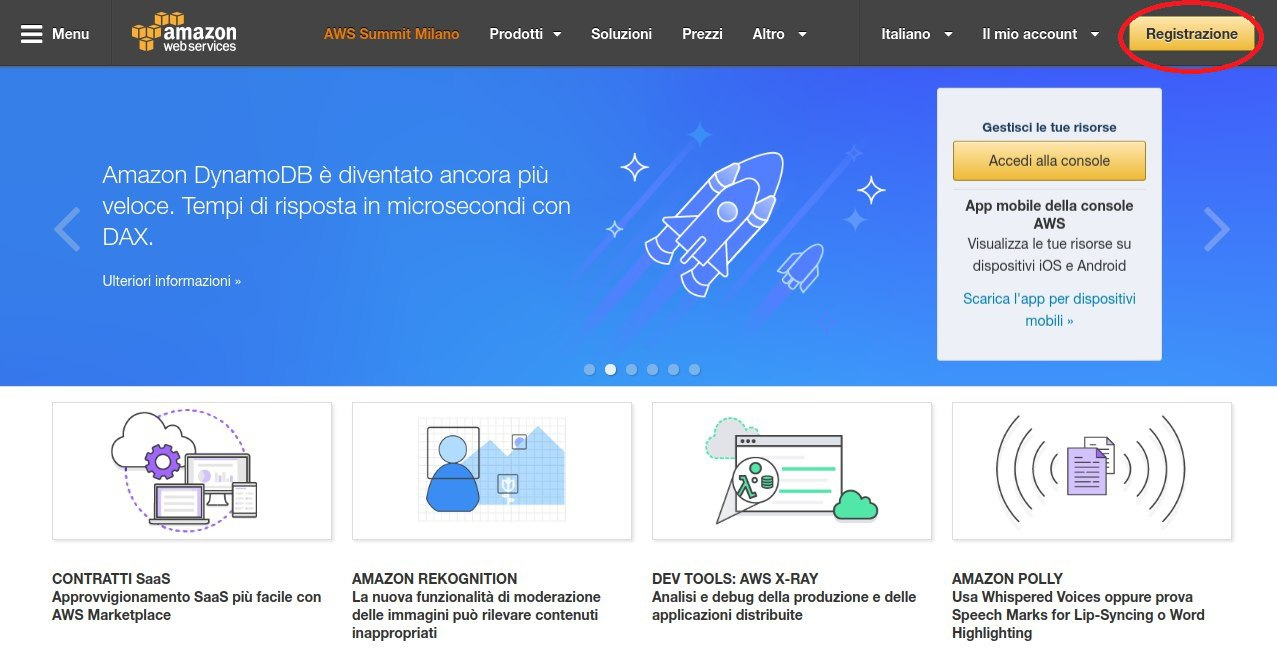
\includegraphics[width=\textwidth,height=\textheight,keepaspectratio]{sezioni/images/aws.jpg}
\caption{Registrazione AWS}
\end{figure}

\subsubsection{Serverless}
Serverless è un framework per alcuni servizi di cloud computing, tra i quali quelli di Amazon Web Services. È un progetto molto giovane, ma che gode già di un ottimo supporto.\\
Esso permette la realizzazione e il deploy dei servizi in maniera molto più facile e veloce, infatti l'effettivo deploy del sistema è semplificato, velocizzato e automatizzato grazie ad esso. \\
È necessario applicare la seguente procedura:
\begin{itemize}
	\item installare il framework lanciando il comando \file{npm install serverless -g} nel terminale;
	\item creare delle AWS Access Key seguendo le istruzioni presenti al link \url{https://serverless.com/framework/docs/providers/aws/guide/credentials#creating-aws-access-keys} (visitato in data 2017-04-28);
	\item fornire le credenziali create seguendo le istruzioni al link \url{https://serverless.com/framework/docs/providers/aws/guide/credentials#setup-with-serverless-config-credentials-command} (visitato in data 2017-04-28);
\end{itemize}
\subsubsection{Microsoft Speaker Recognition}
\subsubsection{IBM Watson Speech to Text}
\subsubsection{api.ai}
\subsection{Configurazione}